\documentclass[11pt,preprint]{elsarticle}

\usepackage{lmodern}
%%%% My spacing
\usepackage{setspace}
\setstretch{1.2}
\DeclareMathSizes{12}{14}{10}{10}

% Wrap around which gives all figures included the [H] command, or places it "here". This can be tedious to code in Rmarkdown.
\usepackage{float}
\let\origfigure\figure
\let\endorigfigure\endfigure
\renewenvironment{figure}[1][2] {
    \expandafter\origfigure\expandafter[H]
} {
    \endorigfigure
}

\let\origtable\table
\let\endorigtable\endtable
\renewenvironment{table}[1][2] {
    \expandafter\origtable\expandafter[H]
} {
    \endorigtable
}


\usepackage{ifxetex,ifluatex}
\usepackage{fixltx2e} % provides \textsubscript
\ifnum 0\ifxetex 1\fi\ifluatex 1\fi=0 % if pdftex
  \usepackage[T1]{fontenc}
  \usepackage[utf8]{inputenc}
\else % if luatex or xelatex
  \ifxetex
    \usepackage{mathspec}
    \usepackage{xltxtra,xunicode}
  \else
    \usepackage{fontspec}
  \fi
  \defaultfontfeatures{Mapping=tex-text,Scale=MatchLowercase}
  \newcommand{\euro}{€}
\fi

\usepackage{amssymb, amsmath, amsthm, amsfonts}

\def\bibsection{\section*{References}} %%% Make "References" appear before bibliography


\usepackage[numbers]{natbib}

\usepackage{longtable}
\usepackage[margin=2.3cm,bottom=2cm,top=2.5cm, includefoot]{geometry}
\usepackage{fancyhdr}
\usepackage[bottom, hang, flushmargin]{footmisc}
\usepackage{graphicx}
\numberwithin{equation}{section}
\numberwithin{figure}{section}
\numberwithin{table}{section}
\setlength{\parindent}{0cm}
\setlength{\parskip}{1.3ex plus 0.5ex minus 0.3ex}
\usepackage{textcomp}
\renewcommand{\headrulewidth}{0pt}

\usepackage{array}
\newcolumntype{x}[1]{>{\centering\arraybackslash\hspace{0pt}}p{#1}}

%%%%  Remove the "preprint submitted to" part. Don't worry about this either, it just looks better without it:
\journal{Journal of Finance}

 \def\tightlist{} % This allows for subbullets!

\usepackage{hyperref}
\hypersetup{breaklinks=true,
            bookmarks=true,
            colorlinks=true,
            citecolor=blue,
            urlcolor=blue,
            linkcolor=blue,
            pdfborder={0 0 0}}


% The following packages allow huxtable to work:
\usepackage{siunitx}
\usepackage{multirow}
\usepackage{hhline}
\usepackage{calc}
\usepackage{tabularx}
\usepackage{booktabs}
\usepackage{caption}


\newenvironment{columns}[1][]{}{}

\newenvironment{column}[1]{\begin{minipage}{#1}\ignorespaces}{%
\end{minipage}
\ifhmode\unskip\fi
\aftergroup\useignorespacesandallpars}

\def\useignorespacesandallpars#1\ignorespaces\fi{%
#1\fi\ignorespacesandallpars}

\makeatletter
\def\ignorespacesandallpars{%
  \@ifnextchar\par
    {\expandafter\ignorespacesandallpars\@gobble}%
    {}%
}
\makeatother


% definitions for citeproc citations
\NewDocumentCommand\citeproctext{}{}
\NewDocumentCommand\citeproc{mm}{%
\href{\#cite.\detokenize{#1}}{#2}\nocite{#1}}

\makeatletter
% allow citations to break across lines
\let\@cite@ofmt\@firstofone
% avoid brackets around text for \cite:
\def\@biblabel#1{}
\def\@cite#1#2{{#1\if@tempswa , #2\fi}}
\makeatother
\newlength{\cslhangindent}
\setlength{\cslhangindent}{1.5em}
\newlength{\csllabelwidth}
\setlength{\csllabelwidth}{3em}
\newenvironment{CSLReferences}[2] % #1 hanging-indent, #2 entry-spacing
{\begin{list}{}{%
	\setlength{\itemindent}{0pt}
	\setlength{\leftmargin}{0pt}
	\setlength{\parsep}{0pt}
	% turn on hanging indent if param 1 is 1
	\ifodd #1
	\setlength{\leftmargin}{\cslhangindent}
	\setlength{\itemindent}{-1\cslhangindent}
	\fi
	% set entry spacing
	\setlength{\itemsep}{#2\baselineskip}}}
{\end{list}}

\usepackage{calc}
\newcommand{\CSLBlock}[1]{\hfill\break\parbox[t]{\linewidth}{\strut\ignorespaces#1\strut}}
\newcommand{\CSLLeftMargin}[1]{\parbox[t]{\csllabelwidth}{\strut#1\strut}}
\newcommand{\CSLRightInline}[1]{\parbox[t]{\linewidth - \csllabelwidth}{\strut#1\strut}}
\newcommand{\CSLIndent}[1]{\hspace{\cslhangindent}#1}


\urlstyle{same}  % don't use monospace font for urls
\setlength{\parindent}{0pt}
\setlength{\parskip}{6pt plus 2pt minus 1pt}
\setlength{\emergencystretch}{3em}  % prevent overfull lines
\setcounter{secnumdepth}{5}

%%% Use protect on footnotes to avoid problems with footnotes in titles
\let\rmarkdownfootnote\footnote%
\def\footnote{\protect\rmarkdownfootnote}
\IfFileExists{upquote.sty}{\usepackage{upquote}}{}

%%% Include extra packages specified by user

%%% Hard setting column skips for reports - this ensures greater consistency and control over the length settings in the document.
%% page layout
%% paragraphs
\setlength{\baselineskip}{12pt plus 0pt minus 0pt}
\setlength{\parskip}{12pt plus 0pt minus 0pt}
\setlength{\parindent}{0pt plus 0pt minus 0pt}
%% floats
\setlength{\floatsep}{12pt plus 0 pt minus 0pt}
\setlength{\textfloatsep}{20pt plus 0pt minus 0pt}
\setlength{\intextsep}{14pt plus 0pt minus 0pt}
\setlength{\dbltextfloatsep}{20pt plus 0pt minus 0pt}
\setlength{\dblfloatsep}{14pt plus 0pt minus 0pt}
%% maths
\setlength{\abovedisplayskip}{12pt plus 0pt minus 0pt}
\setlength{\belowdisplayskip}{12pt plus 0pt minus 0pt}
%% lists
\setlength{\topsep}{10pt plus 0pt minus 0pt}
\setlength{\partopsep}{3pt plus 0pt minus 0pt}
\setlength{\itemsep}{5pt plus 0pt minus 0pt}
\setlength{\labelsep}{8mm plus 0mm minus 0mm}
\setlength{\parsep}{\the\parskip}
\setlength{\listparindent}{\the\parindent}
%% verbatim
\setlength{\fboxsep}{5pt plus 0pt minus 0pt}



\begin{document}



\begin{frontmatter}  %

\title{US Baby Names}

% Set to FALSE if wanting to remove title (for submission)




\author[Add1]{Anya Nash}
\ead{25051911@sun.ac.za}





\address[Add1]{Stellenbosch University, Stellenbosch, South Africa}



\vspace{1cm}





\vspace{0.5cm}

\end{frontmatter}

\setcounter{footnote}{0}



%________________________
% Header and Footers
%%%%%%%%%%%%%%%%%%%%%%%%%%%%%%%%%
\pagestyle{fancy}
\chead{}
\rhead{}
\lfoot{}
\rfoot{}
\lhead{}
%\rfoot{\footnotesize Page \thepage } % "e.g. Page 2"
\cfoot{}

%\setlength\headheight{30pt}
%%%%%%%%%%%%%%%%%%%%%%%%%%%%%%%%%
%________________________

\headsep 35pt % So that header does not go over title




\subsection{Spearman Correlation by
Year}\label{spearman-correlation-by-year}

\subsubsection{Spearman Correlation for Female
Names}\label{spearman-correlation-for-female-names}

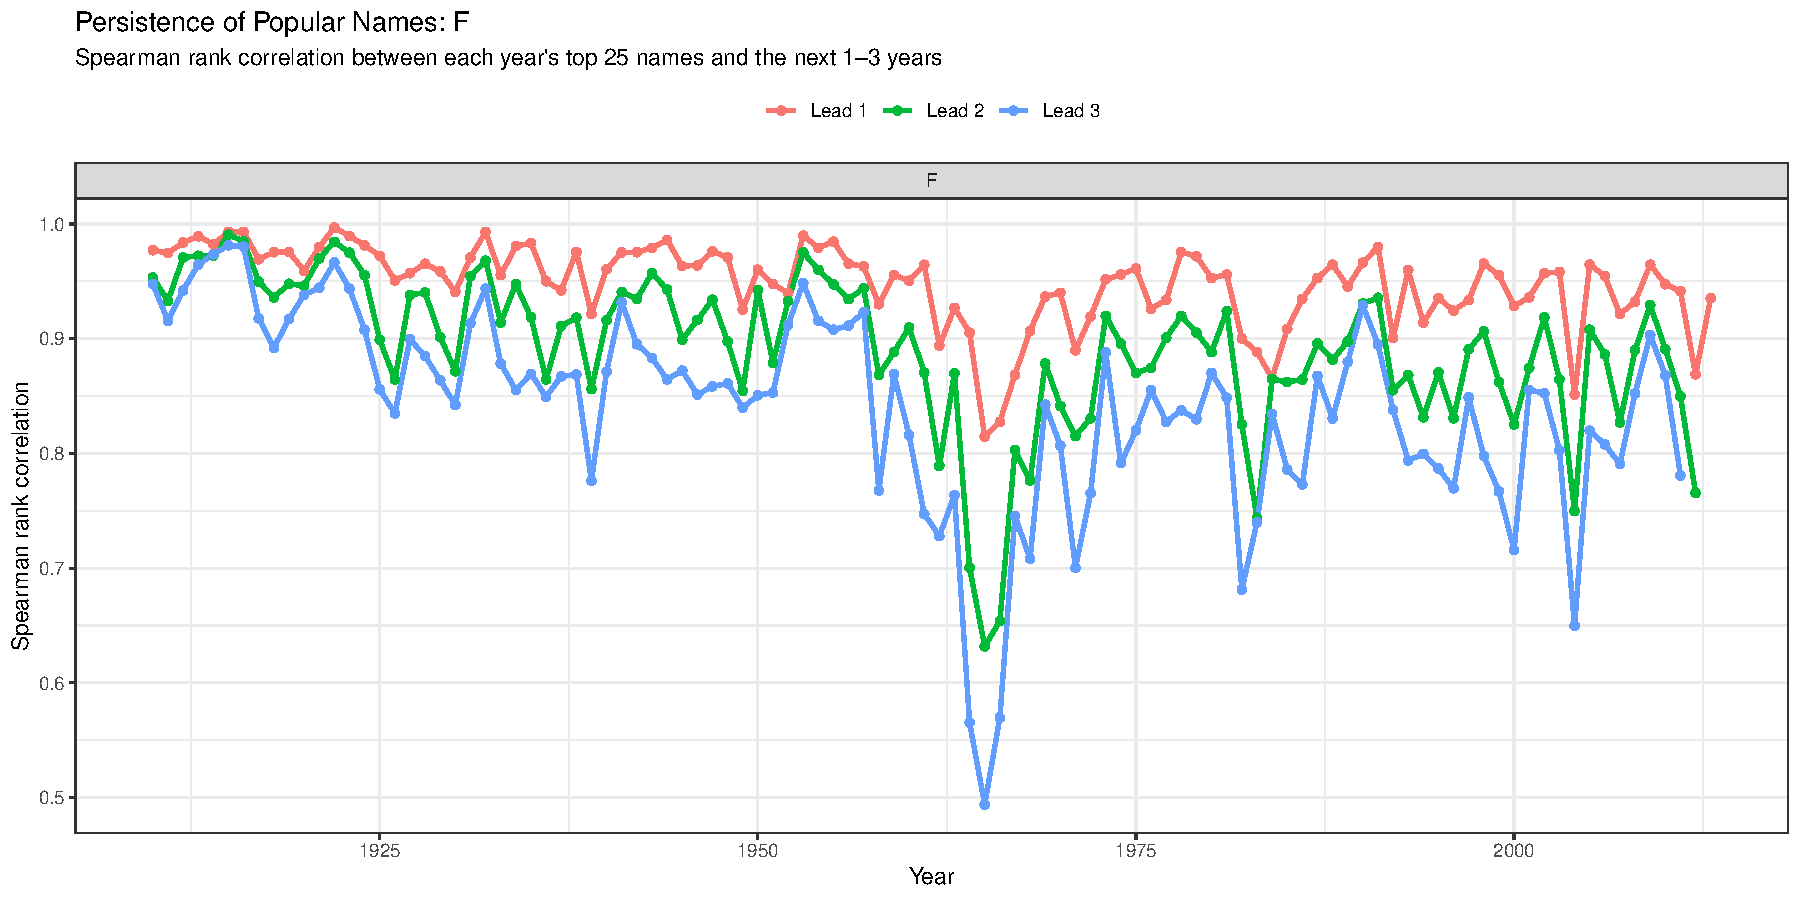
\includegraphics[width=1\linewidth]{25051911_Question_2_files/figure-latex/unnamed-chunk-4-1}
The graph shows that the top 25 female names are very persistent for the
time period analysed. For most of the years, the Spearman rank
correlation is between 0.8 and 1, except for between 1960 and 1970,
around 1985 and around 2005. Therefore, if a female name is in the top
25, then there is a very high probability that it will be in the top 25
in the following year as well as the year after that. According to this
graph, it appears that female names are no more or less likely to
persist since the 1990s compared to earlier years; the pattern does not
appear to change significantly from the 1990s.

\subsubsection{Spearman Correlation for Male
Names}\label{spearman-correlation-for-male-names}

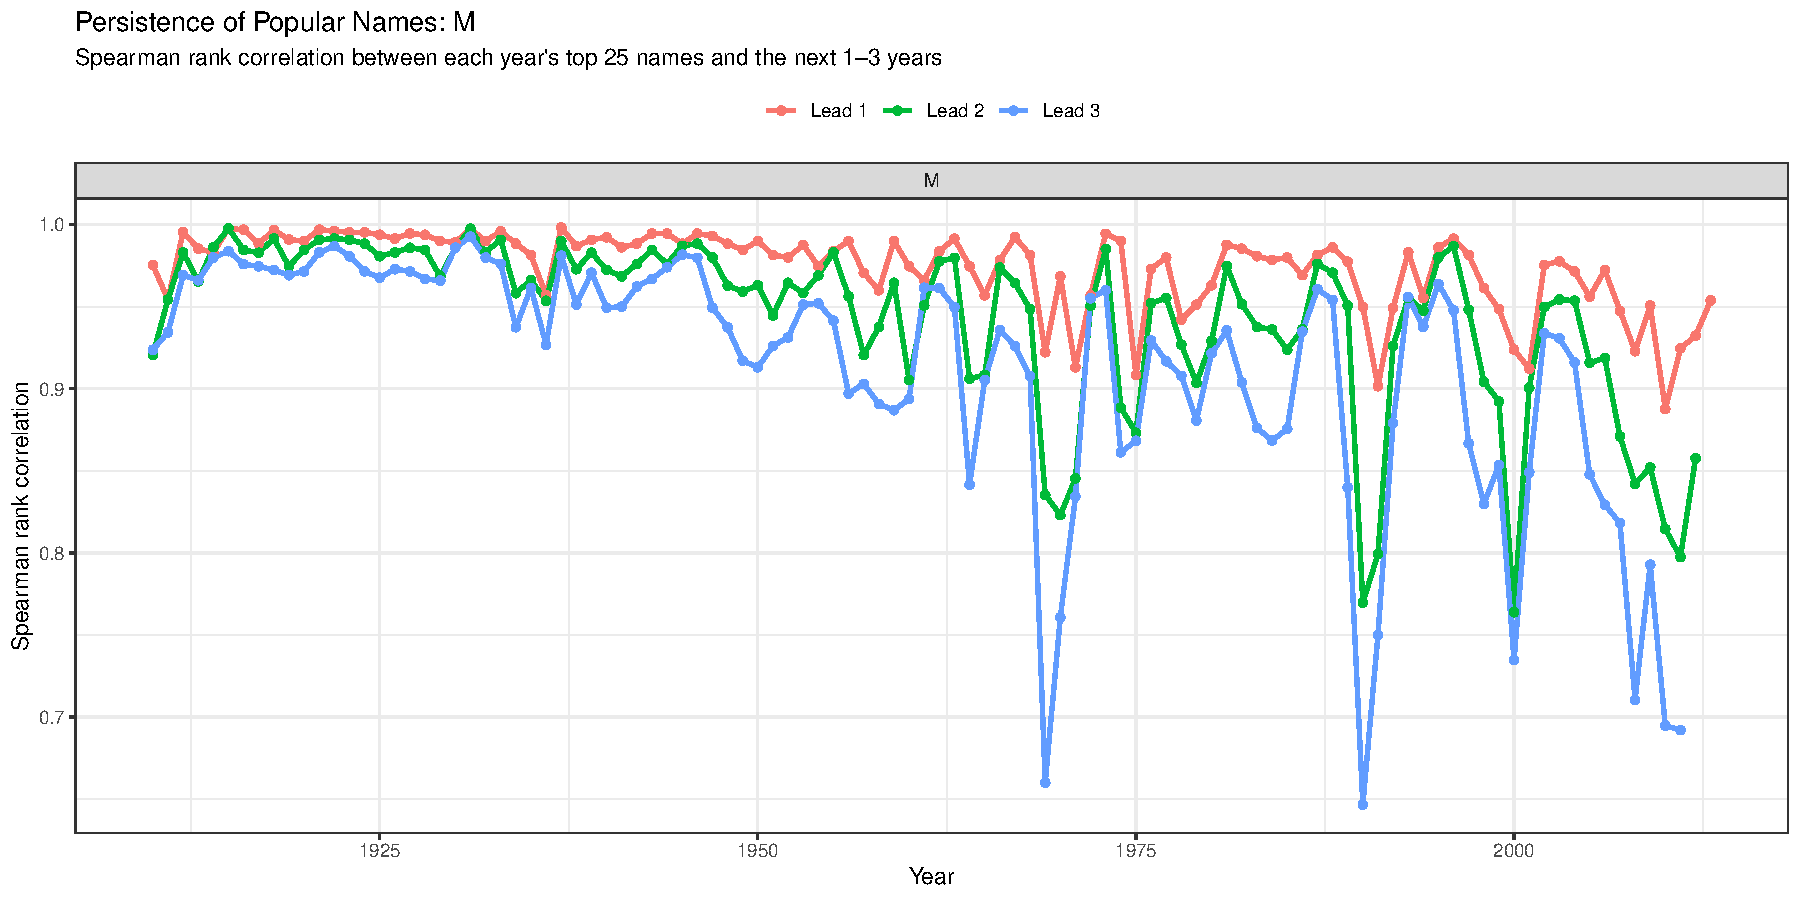
\includegraphics[width=1\linewidth]{25051911_Question_2_files/figure-latex/unnamed-chunk-5-1}

The graph shows that the top 25 male names are very persistent for the
time period analysed. Before 1965, the Spearman rank correlation remains
between 0.85 and 1, however, the range significantly increases and the
consistency decreases after 1965. This indicates that male names were
initially quite persistent, but that persistence has decreased
significantly since 1965. Therefore, the probability of a male name
remaining in the top 25 male names began very high, but in more recent
years, that probability has become smaller. From this graph, it appears
that male names are less persistent since the 1990s than prior to that -
popular names have become a bit slower to persist since the 1990s.

\subsection{Spearman Correlation by
Decade}\label{spearman-correlation-by-decade}

\subsubsection{Spearman Correlation by Decade for Female
Names}\label{spearman-correlation-by-decade-for-female-names}

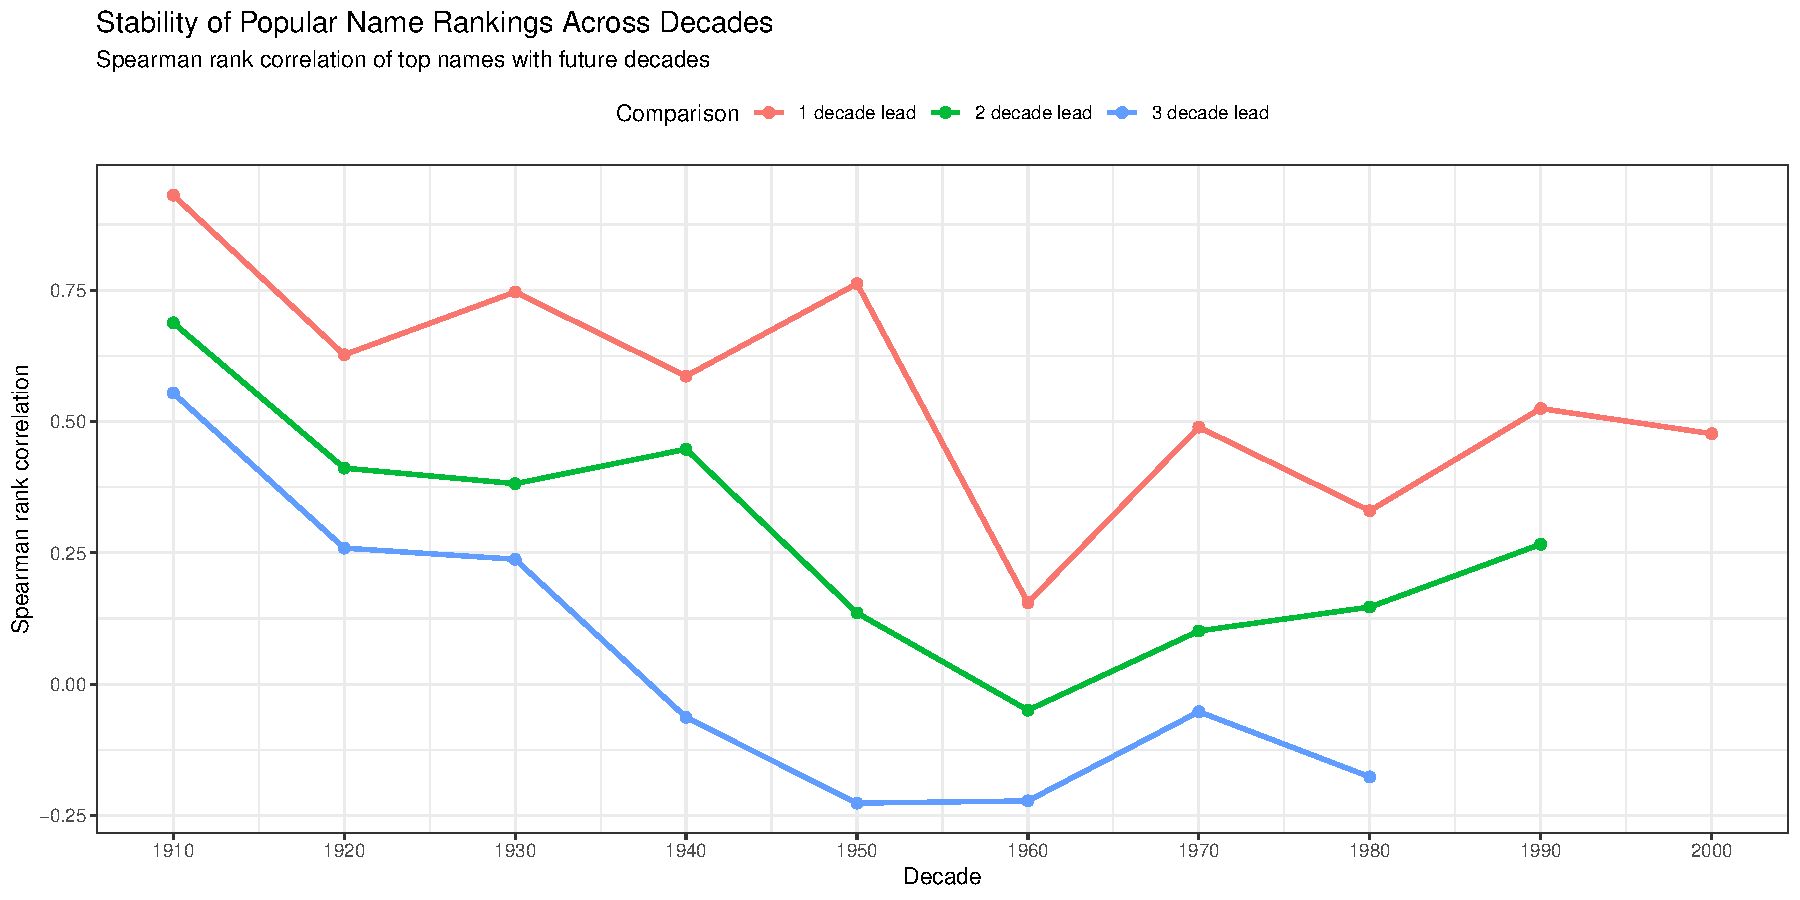
\includegraphics[width=1\linewidth]{25051911_Question_2_files/figure-latex/unnamed-chunk-7-1}

The same trends are apparent when looking at popular female names by
decade - according to this graph, it appears that female names are no
more or less likely to persist since the 1990s compared to earlier
years; the pattern does not appear to change significantly from the
1990s.

\subsubsection{Spearman Correlation by Decade for Male
Names}\label{spearman-correlation-by-decade-for-male-names}

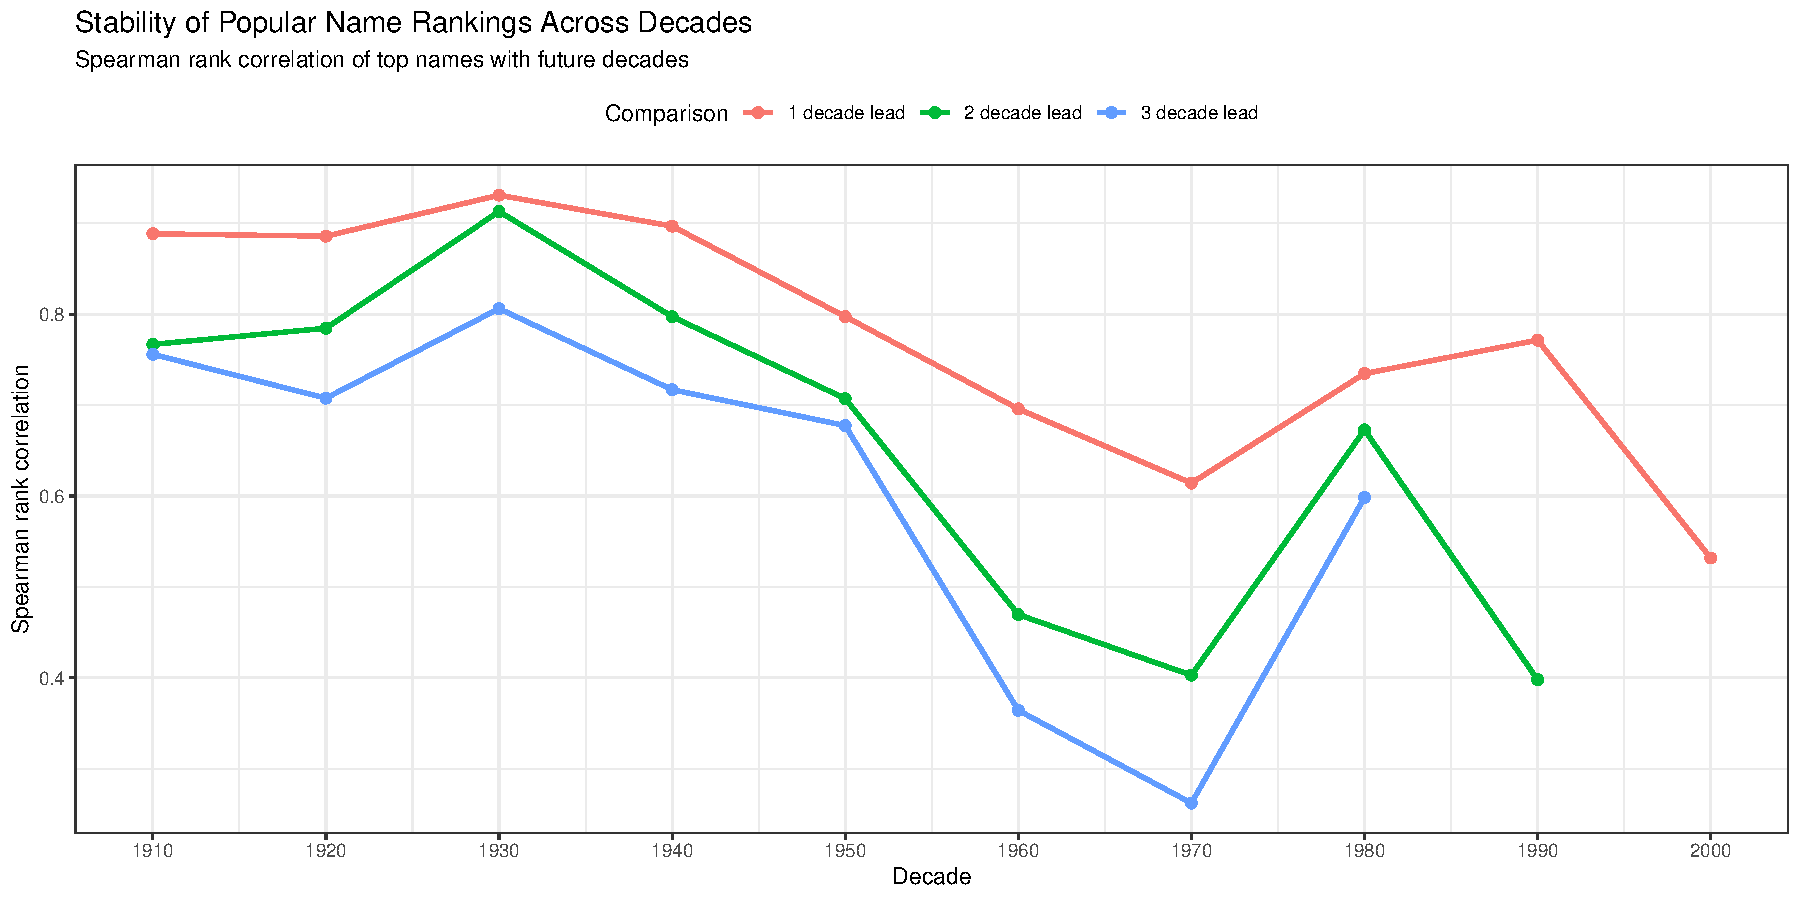
\includegraphics[width=1\linewidth]{25051911_Question_2_files/figure-latex/unnamed-chunk-8-1}

Once again, this graph shows similar trends to the yearly popular make
names graph above. From this graph, it appears that male names are less
persistent since the 1990s than prior to that - popular names have
become a bit slower to persist since the 1990s.

\subsection{Names Surge}\label{names-surge}

The table below shows the top 10 female names and top 10 male names that
experienced the largest year-to-year percentage rank improvement. The
table excludes names with an initial count of less than 100, so that the
rank improvement is not driven by relative large changes in very
unpopular names.

\begin{longtable}[]{@{}
  >{\raggedright\arraybackslash}p{(\linewidth - 18\tabcolsep) * \real{0.0382}}
  >{\raggedright\arraybackslash}p{(\linewidth - 18\tabcolsep) * \real{0.0534}}
  >{\raggedright\arraybackslash}p{(\linewidth - 18\tabcolsep) * \real{0.0916}}
  >{\raggedright\arraybackslash}p{(\linewidth - 18\tabcolsep) * \real{0.1145}}
  >{\raggedright\arraybackslash}p{(\linewidth - 18\tabcolsep) * \real{0.1069}}
  >{\raggedright\arraybackslash}p{(\linewidth - 18\tabcolsep) * \real{0.1221}}
  >{\raggedright\arraybackslash}p{(\linewidth - 18\tabcolsep) * \real{0.1374}}
  >{\raggedright\arraybackslash}p{(\linewidth - 18\tabcolsep) * \real{0.1069}}
  >{\raggedright\arraybackslash}p{(\linewidth - 18\tabcolsep) * \real{0.0992}}
  >{\raggedright\arraybackslash}p{(\linewidth - 18\tabcolsep) * \real{0.1298}}@{}}
\caption{Top 10 year-on-year name surges by gender}\tabularnewline
\toprule\noalign{}
\begin{minipage}[b]{\linewidth}\raggedright
Year
\end{minipage} & \begin{minipage}[b]{\linewidth}\raggedright
Gender
\end{minipage} & \begin{minipage}[b]{\linewidth}\raggedright
Name
\end{minipage} & \begin{minipage}[b]{\linewidth}\raggedright
Previous count
\end{minipage} & \begin{minipage}[b]{\linewidth}\raggedright
Current count
\end{minipage} & \begin{minipage}[b]{\linewidth}\raggedright
Change in count
\end{minipage} & \begin{minipage}[b]{\linewidth}\raggedright
\% change in count
\end{minipage} & \begin{minipage}[b]{\linewidth}\raggedright
Previous rank
\end{minipage} & \begin{minipage}[b]{\linewidth}\raggedright
Current rank
\end{minipage} & \begin{minipage}[b]{\linewidth}\raggedright
Rank improvement
\end{minipage} \\
\midrule\noalign{}
\endfirsthead
\toprule\noalign{}
\begin{minipage}[b]{\linewidth}\raggedright
Year
\end{minipage} & \begin{minipage}[b]{\linewidth}\raggedright
Gender
\end{minipage} & \begin{minipage}[b]{\linewidth}\raggedright
Name
\end{minipage} & \begin{minipage}[b]{\linewidth}\raggedright
Previous count
\end{minipage} & \begin{minipage}[b]{\linewidth}\raggedright
Current count
\end{minipage} & \begin{minipage}[b]{\linewidth}\raggedright
Change in count
\end{minipage} & \begin{minipage}[b]{\linewidth}\raggedright
\% change in count
\end{minipage} & \begin{minipage}[b]{\linewidth}\raggedright
Previous rank
\end{minipage} & \begin{minipage}[b]{\linewidth}\raggedright
Current rank
\end{minipage} & \begin{minipage}[b]{\linewidth}\raggedright
Rank improvement
\end{minipage} \\
\midrule\noalign{}
\endhead
\bottomrule\noalign{}
\endlastfoot
1976 & F & Jaime & 897 & 7836 & 6939 & 773.6 & 262 & 29 & 803.4483 \\
1989 & F & Kiara & 171 & 2595 & 2424 & 1417.5 & 832 & 115 & 623.4783 \\
2002 & F & Ashanti & 253 & 2927 & 2674 & 1056.9 & 784 & 115 &
581.7391 \\
1957 & F & Tammy & 204 & 4363 & 4159 & 2038.7 & 602 & 107 & 462.6168 \\
1979 & F & Brianne & 133 & 1655 & 1522 & 1144.4 & 813 & 168 &
383.9286 \\
1995 & F & Alondra & 111 & 1149 & 1038 & 935.1 & 1121 & 242 &
363.2231 \\
2007 & F & Miley & 141 & 1213 & 1072 & 760.3 & 1249 & 277 & 350.9025 \\
1966 & F & Michelle & 16215 & 27152 & 10937 & 67.4 & 18 & 4 &
350.0000 \\
1991 & F & Iesha & 253 & 1875 & 1622 & 641.1 & 703 & 157 & 347.7707 \\
1982 & F & Kayla & 266 & 2268 & 2002 & 752.6 & 583 & 132 & 341.6667 \\
2011 & M & Mason & 14831 & 19488 & 4657 & 31.4 & 12 & 2 & 500.0000 \\
2013 & M & Jayceon & 128 & 1827 & 1699 & 1327.3 & 1059 & 208 &
409.1346 \\
2010 & M & Bentley & 497 & 3762 & 3265 & 656.9 & 505 & 100 & 405.0000 \\
1998 & M & Dawson & 141 & 1883 & 1742 & 1235.5 & 779 & 175 & 345.1429 \\
2013 & M & Noah & 17302 & 18179 & 877 & 5.1 & 4 & 1 & 300.0000 \\
1995 & M & Tristan & 441 & 3085 & 2644 & 599.5 & 454 & 121 & 275.2066 \\
2013 & M & Jase & 1100 & 4539 & 3439 & 312.6 & 304 & 89 & 241.5730 \\
2002 & M & Ethan & 17959 & 22105 & 4146 & 23.1 & 17 & 5 & 240.0000 \\
1995 & M & Bailey & 112 & 990 & 878 & 783.9 & 853 & 273 & 212.4542 \\
1972 & M & Christopher & 48251 & 52195 & 3944 & 8.2 & 6 & 2 &
200.0000 \\
\end{longtable}

\subsection{Names Surge and TV Shows/
Movies}\label{names-surge-and-tv-shows-movies}

\subsubsection{Male Names}\label{male-names}

The plot below shows how the popularity and persistence of male names
interacts with character names of TV show or movie characters. The male
names chosen are the 20 male names that experienced the largest
percentage rank improvement. These names were then merged with character
names.

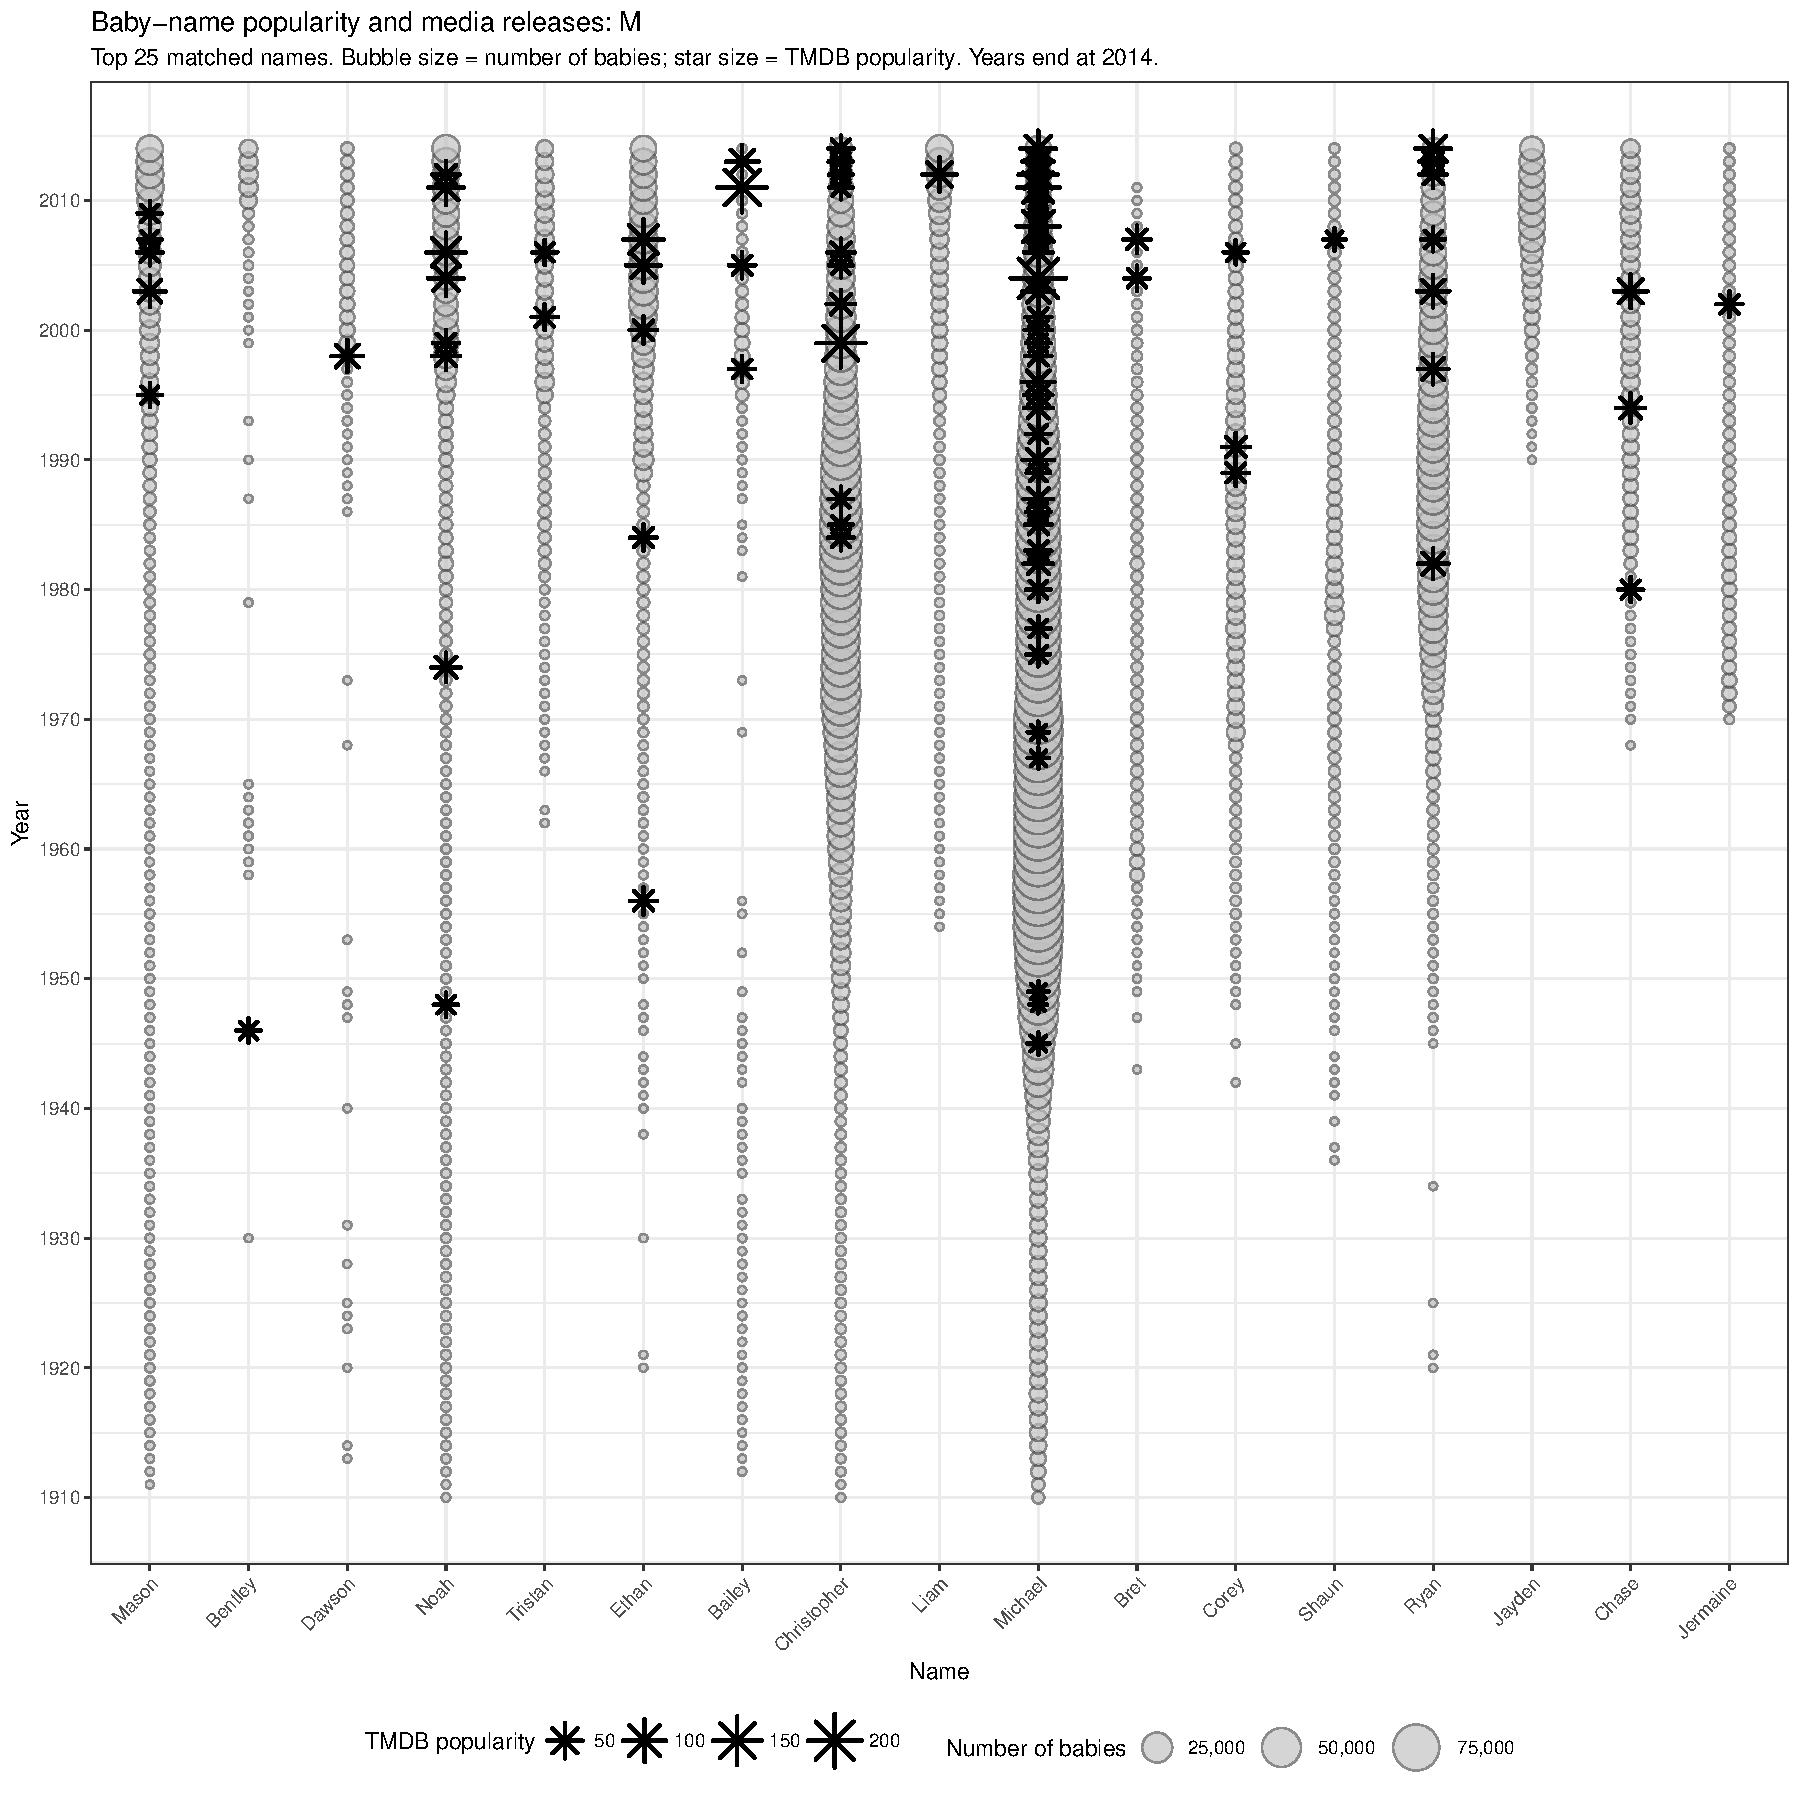
\includegraphics[width=1\linewidth]{25051911_Question_2_files/figure-latex/unnamed-chunk-14-1}

As seen from the plot above, there is not a clear pattern between the
popularity or persistence of names and character names from TV shows/
movies for these particular male names. However, it is interesting to
observe how these variables develop and interact over time. Also, for
most of these names, their popularity has been increasing over time.
This makes them an excellent choice for a toy company, because their
popularity is increasing, and increasing regardless of popular character
names. It is clear that some names are classics - Christopher, Michael
and Ryan remain persistently popular, regardless of whether TV show or
movie characters have these names. These names are also the names of
characters in many TV shows/ movies. Therefore, for a toy company, these
names are good to take note of, because they are unlikely to change
significantly in popularity over time, meaning they are a lower-risk
investment.

\subsubsection{Female Names}\label{female-names}

The plot below shows how the popularity and persistence of female names
interacts with character names of TV show or movie characters. The
female names chosen are the 20 female names that experienced the largest
percentage rank improvement. These names were then merged with character
names.

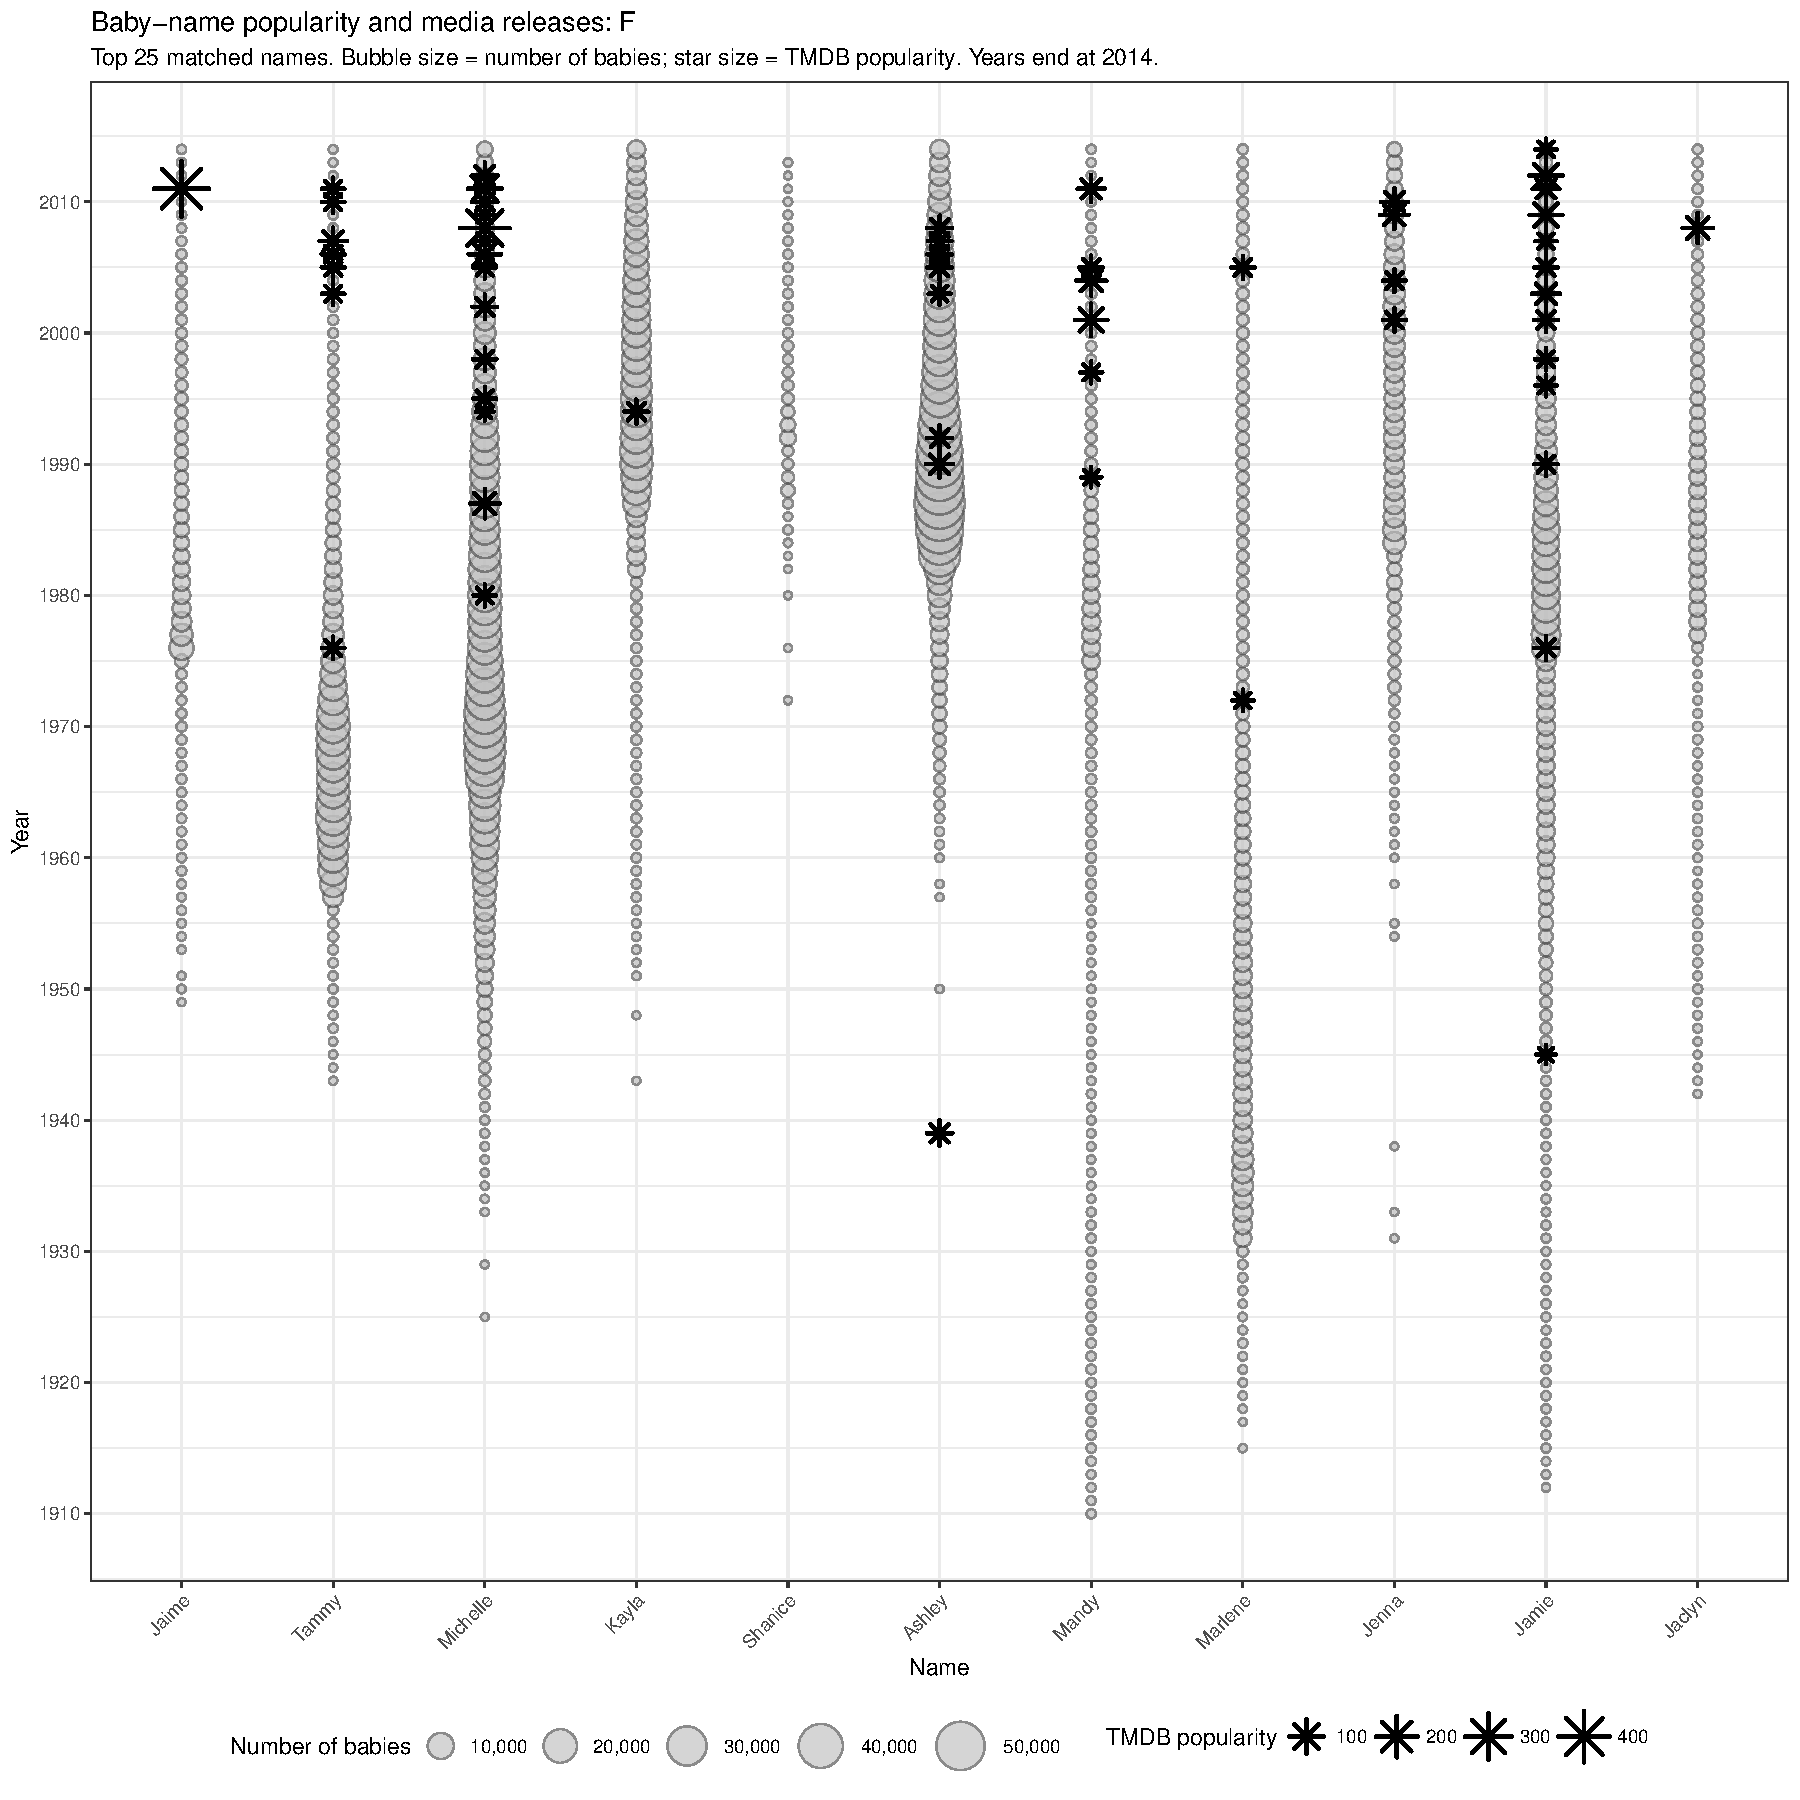
\includegraphics[width=1\linewidth]{25051911_Question_2_files/figure-latex/unnamed-chunk-15-1}

As seen from the plot above, there is not a clear pattern between the
popularity or persistence of names and character names from TV shows/
movies for these particular female names. However, it is interesting to
observe how these variables develop and interact over time. It is clear
that some names are classics - Michelle, Kayla, Ashley, Jenna and Jamie
remain persistently popular, regardless of whether TV show or movie
characters have these names. Therefore, for a toy company, these names
are good to take note of, because they are unlikely to change
significantly in popularity over time, meaning they are a lower-risk
investment.

\bibliography{Tex/ref}





\end{document}
